% questions.tex —— 2021 年·上海春季招生数学试卷 · 题目内容片段（无答案）
% 由 tools/generate_projects.py 依来源总账自 2021/2021_数学真题_春季上海_试题.md 生成，勿手改（改源 MD 后重跑）


\begin{gktip}
\textbf{来源说明}：题面依据固定 PDF 第 1–3 页转录；该副本首页注明“网络收集版”，不据此认证出版者、版次、传播链或官方身份。全卷已有独立推导，Q9 定义约定及 Q12 原题量词与副本参考解的矛盾保持待核；不把卷内参考解称为官方答案。

\textbf{页码映射}：Q1–14 在 PDF 第 1 页，Q15–21 在第 2–3 页（Q21 延续至第 3 页）。固定副本未见分值或考试时长标注。Q17 原图已按固定 PDF 第 2 页重绘为 TikZ，保留可见拓扑与虚实线，坐标仅作投影示意。
\end{gktip}

\gkpart{一、填空题}

\begin{question}
\gkti{1}等差数列 $\{a_n\}$ 中，$a_1=3,d=2$，则 $a_{10}=\underline{\quad}$。

\end{question}
\begin{question}
\gkti{2}已知复数 $z$ 满足 $z=1-3i$（$i$ 是虚数单位），则 $|\bar z-i|=\underline{\quad}$。

\end{question}
\begin{question}
\gkti{3}不等式 $\frac{2x+5}{x-2}<1$ 的解集为\gkblank{}。

\end{question}
\begin{question}
\gkti{4}已知圆柱的底面半径为 1，母线长为 2，则其侧面积为\gkblank{}。

\end{question}
\begin{question}
\gkti{5}求直线 $x=-2$ 与直线 $\sqrt3x-y+1=0$ 的夹角为\gkblank{}。

\end{question}
\begin{question}
\gkti{6}方程组 $\begin{cases}a_1x+b_1y=c_1\\a_2x+b_2y=c_2\end{cases}$ 无解，求 $\begin{vmatrix}a_1&b_1\\a_2&b_2\end{vmatrix}=\underline{\quad}$。

\end{question}
\begin{question}
\gkti{7}$(x+1)^n$ 的二项展开式中有且仅有 $x^3$ 的系数为最大值，则 $x^3$ 的系数为\gkblank{}。

\end{question}
\begin{question}
\gkti{8}已知函数 $f(x)=3^x+\frac a{3^x+1}$（$a>0$）的最小值为 5，则 $a=$\gkblank{}。

\end{question}
\begin{question}
\gkti{9}在无穷等比数列 $\{a_n\}$ 中，$\lim_{n\to\infty}(a_1-a_n)=4$，则 $a_2$ 的取值范围是\gkblank{}。

\end{question}
\begin{question}
\gkti{10}某人某天需要运动总时长大于等于 60 分钟，现有五项运动可以选择，如下表所示，问有几种运动方式组合\gkblank{}。

\begin{center}
\begin{tabular}{lllll}
\toprule
A运动 & B运动 & C运动 & D运动 & E运动 \\
\midrule
7点－8点 & 8点－9点 & 9点－10点 & 10点－11点 & 11点－12点 \\
30分钟 & 20分钟 & 40分钟 & 30分钟 & 30分钟 \\
\bottomrule
\end{tabular}
\end{center}

\end{question}
\begin{question}
\gkti{11}已知椭圆 $x^2+\frac{y^2}{b^2}=1$（$0<b<1$）的左、右焦点为 $F_1,F_2$，以 $O$ 为顶点，$F_2$ 为焦点作抛物线交椭圆于 $P$，且 $\angle PF_1F_2=45^\circ$，则抛物线的准线方程是\gkblank{}。

\end{question}
\begin{question}
\gkti{12}已知 $\theta>0$，对任意 $n\in\mathbb N^*$，总存在实数 $\varphi$，使得 $\cos(n\theta+\varphi)<\frac{\sqrt3}{2}$，则 $\theta$ 的最小值是\gkblank{}。

\end{question}
\gkpart{二、单选题}

\begin{question}
\gkti{13}下列函数中，在定义域内存在反函数的是（ ）。A. $x^2$；B. $\sin x$；C. $2^x$；D. $y=1$。

\end{question}
\begin{question}
\gkti{14}已知集合 $A=\{x\mid x^2-x-2\ge0\}$，$B=\{x\mid x>-1\}$，则（ ）。A. $A\subseteq B$；B. $C_R A\subseteq C_R B$；C. $A\cap B=\phi$；D. $A\cup B=R$。

\end{question}
\begin{question}
\gkti{15}已知函数 $y=f(x)$ 的定义域为 $\mathbf R$，下列是 $f(x)$ 无最大值的充分条件是（ ）。A. $f(x)$ 为偶函数且关于直线 $x=1$ 对称；B. $f(x)$ 为偶函数且关于点 $(1,1)$ 对称；C. $f(x)$ 为奇函数且关于直线 $x=1$ 对称；D. $f(x)$ 为奇函数且关于点 $(1,1)$ 对称。

\end{question}
\begin{question}
\gkti{16}在 $\triangle ABC$ 中，$D$ 为 $BC$ 中点，$E$ 为 $AD$ 中点，则以下结论：①存在 $\triangle ABC$，使得 $\overrightarrow{AB}\cdot\overrightarrow{CE}=0$；②存在三角形 $\triangle ABC$，使得 $\overrightarrow{CE}\parallel(\overrightarrow{CB}+\overrightarrow{CA})$，则（ ）。A. ①成立，②成立；B. ①成立，②不成立；C. ①不成立，②成立；D. ①不成立，②不成立。

\end{question}
\gkpart{三、解答题}

\Needspace{0.4\textheight}
\begin{question}
\gkti{17}四棱锥 $P-ABCD$，底面为正方形 $ABCD$，边长为 4，$E$ 为 $AB$ 中点，$PE\perp$ 平面 $ABCD$。

（1） 若 $\triangle PAB$ 为等边三角形，求四棱锥 $P-ABCD$ 的体积；

（2） 若 $CD$ 的中点为 $F$，$PF$ 与平面 $ABCD$ 所成角为 $45^\circ$，求 $PD$ 与 $AC$ 所成角的大小。
\nopagebreak[4]
\begin{center}% 2021 上海春季卷第 17 题；按固定副本第 2 页重绘可见拓扑与线型，坐标仅作投影示意。
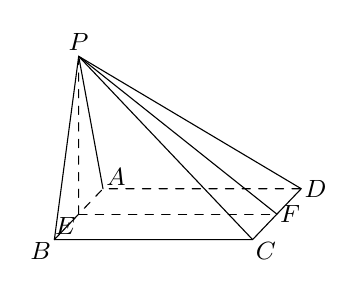
\begin{tikzpicture}[scale=.95,line cap=round,line join=round,font=\small]
  \coordinate (A) at (.65,.68);
  \coordinate (B) at (0,0);
  \coordinate (C) at (2.65,0);
  \coordinate (D) at (3.30,.68);
  \coordinate (E) at (.325,.34);
  \coordinate (F) at (2.975,.34);
  \coordinate (P) at (.325,2.45);

  \draw[dashed] (P) -- (E) -- (A) -- (D);
  \draw[dashed] (E) -- (F);
  \draw (P) -- (A);
  \draw (P) -- (B) -- (E);
  \draw (P) -- (D);
  \draw (P) -- (C);
  \draw (P) -- (F);
  \draw (B) -- (C) -- (F) -- (D);

  \node[above,inner sep=2pt] at (P) {$P$};
  \node[above right,inner sep=1pt] at (A) {$A$};
  \node[below left,inner sep=1pt] at (B) {$B$};
  \node[below right,inner sep=1pt] at (C) {$C$};
  \node[right,inner sep=1pt] at (D) {$D$};
  \node[below left,inner sep=1pt] at (E) {$E$};
  \node[right,inner sep=1pt] at (F) {$F$};
\end{tikzpicture}
\end{center}
\nopagebreak[4]
\end{question}
\begin{question}
\gkti{18}已知 $A,B,C$ 为 $\triangle ABC$ 的三个内角，$a,b,c$ 是其三条边，$a=2,\cos C=-\frac14$。

（1） 若 $\sin A=2\sin B$，求 $b,c$；

（2） 若 $\cos(A-\frac\pi4)=\frac45$，求 $c$。
\end{question}
\begin{question}
\gkti{19}

（1） 团队在 $O$ 点西侧、东侧 20 千米处设有 $A,B$ 两站点，测量距离发现一点 $P$ 满足 $|PA|-|PB|=20$ 千米，可知 $P$ 在 $A,B$ 为焦点的双曲线上，以 $O$ 点为原点，东侧为 $x$ 轴正半轴，北侧为 $y$ 轴正半轴，建立平面直角坐标系，$P$ 在北偏东 $60^\circ$ 处，求双曲线标准方程和 $P$ 点坐标。

（2） 团队又在南侧、北侧 15 千米处设有 $C,D$ 两站点，测量距离发现 $|QA|-|QB|=30$ 千米，$|QC|-|QD|=10$ 千米，求 $|OQ|$（精确到 1 米）和 $Q$ 点位置（精确到 1 米，$1^\circ$）。
\end{question}
\begin{question}
\gkti{20}已知函数 $f(x)=\sqrt{|x+a|-a}-x$。

（1） 若 $a=1$，求函数的定义域；

（2） 若 $a\ne0$，若 $f(ax)=a$ 有 2 个不同实数根，求 $a$ 的取值范围；

（3） 是否存在实数 $a$，使得函数 $f(x)$ 在定义域内具有单调性？若存在，求出 $a$ 的取值范围。
\end{question}
\begin{question}
\gkti{21}已知数列 $\{a_n\}$ 满足 $a_n\ge0$，对任意 $n\ge2$，$a_n$ 和 $a_{n+1}$ 中存在一项使其为另一项与 $a_{n-1}$ 的等差中项。

（1） 已知 $a_1=5,a_2=3,a_4=2$，求 $a_3$ 的所有可能取值；

（2） 已知 $a_1=a_4=a_7=0$，$a_2,a_5,a_8$ 为正数，求证：$a_2,a_5,a_8$ 成等比数列，并求出公比 $q$；

（3） 已知数列中恰有 3 项为 0，即 $a_r=a_s=a_t=0$，$2<r<s<t$，且 $a_1=1,a_2=2$，求 $a_{r+1}+a_{s+1}+a_{t+1}$ 的最大值。

\end{question}